\def\shft#1{\stackunder[0.5cm]{}{#1}}
\section{Applikationsprotokolle}
\subsection{HTTP-Server und -Client SocketContext}

\begin{frame}{HTTP-Server- und -Client-\texttt{SocketContext}s}{Applikationsprotokolle}
  \begin{center}
    \begin{figure}
    \par\bigskip
    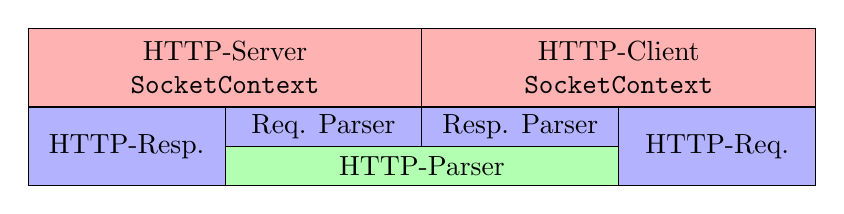
\begin{tikzpicture}
      \draw node [anchor=south, outer sep=0, inner sep=0, draw, fill=green!30, minimum width=5cm, minimum height=0.5cm] (http-p) {HTTP-Parser};

      \draw (http-p.south west) node[anchor=south east, outer sep=0, inner sep=0, draw, fill=blue!30, minimum width=2.5cm, minimum height=1cm] (http-res) {HTTP-Resp.};

      \draw (http-p.south east) node[anchor=south west, outer sep=0, inner sep=0, draw, fill=blue!30, minimum width=2.5cm, minimum height=1cm] (http-res) {HTTP-Req.};

      \draw (http-p.north west) node[anchor=south west, outer sep=0, inner sep=0, draw, fill=blue!30, minimum width=2.5cm, minimum height=0.5cm] (http-reqp) {Req. Parser};

      \draw (http-p.north east) node[anchor=south east, outer sep=0, inner sep=0, draw, fill=blue!30, minimum width=2.5cm, minimum height=0.5cm] (http-respp) {Resp. Parser};

      \draw (http-respp.north west) node[outer sep=0, inner sep=0, anchor=south west, fill=red!30, draw, minimum width=5cm, minimum height=1cm, align=center] (http-c) {HTTP-Client\\ \texttt{SocketContext}};

      \draw (http-reqp.north east) node[outer sep=0, inner sep=0, anchor=south east, fill=red!30, draw, minimum width=5cm, minimum height=1cm, align=center] (http-s) {HTTP-Server\\ \texttt{SocketContext}};
    \end{tikzpicture}
    \caption{HTTP-Server/Client-\texttt{SocketContext} im Detail}
  \end{figure}
  \end{center}
  \begin{itemize}
    \item HTTP-\alert{Requestparser} (ziemlich vollständig)
    \item HTTP-\alert{Responseparser} (ziemlich vollständig)
    \item \alert{Cookie}- und \alert{Query} Support
    \item Connection-Management (Connection: close, keep-alive, upgrade, ...)
    \item echtes \alert{Pipelining} (wird aber wahrscheinlich wieder raus fliegen)
    \item \alert{Payload}-Handling (Body)
  \end{itemize}
\end{frame}
